\documentclass[a4paper]{article}

%% Useful packages
\usepackage{amsmath}
\usepackage{graphicx}	
\usepackage{algpseudocode}
\usepackage{algorithm}
\usepackage[colorinlistoftodos]{todonotes}
\usepackage[colorlinks=true, allcolors=black]{hyperref}
\usepackage[fontsize=11pt]{scrextend}
\usepackage{titlesec}
\usepackage[section]{placeins}
\usepackage{array}
\newcolumntype{L}[1]{>{\raggedright\let\newline\\\arraybackslash\hspace{0pt}}m{#1}}

\setlength\parindent{0pt}
\titleformat*{\section}{\Large\bfseries}
\titleformat*{\subsection}{\Large\bfseries}

\title{PowerEnjoy Service - Integration Test Plan Document}

\begin{document}

\begin{titlepage}
\begin{figure}
\centering

\includegraphics[width=0.2\textwidth]{polimi.jpg}
\par
\LARGE Politecnico di Milano
\end{figure}


\maketitle
\textbf{Version 1.1}
\newline

\raggedright
Authors:
\begin{itemize}
	\item Domenico FAVARO (Mat. 837995)
        	\item Matheus FIM (Mat. 876069)
	\item Caio ZULIANI (Mat. 877266)	
\end{itemize}
\raggedleft
Prof. Elisabetta DI NITTO
\thispagestyle{empty}
\end{titlepage}

\tableofcontents
\newpage
 
\section{Introduction}
\subsection{Revision History}
This section records all revisions to the Document.
\newline \newline
\begin{tabular}{ | c | c | c | c | }
\hline
	Version & Date & Authors & Summary \\ \hline
	1.1 & 15/01/16 & Domenico Favaro, Caio Zuliani, Matheus Fim & Initial Release  \\ \hline
\end{tabular}

\subsection{Purpose and Scope}
The Integration Test Plan Document (ITPD) serves to present the integration sequence and testing for all Subsystems and Components that conform PowerEnjoy Car Sharing Service. This is a key part to guarantee the functioning and quality of the software. The Document will present the division of the System in Subsystems and Components that will endure individual testing as independent modules and then be subject to integration on the whole System.

\subsection{Definitions and Abbreviations}
\begin{itemize}
\item \textbf{RASD:} Reqirements And Specifications Document.
\item \textbf{DD:} Design Document.
\item \textbf{ITPD:} Integration Test Plan Document.
\item \textbf{SDK:} Software Development Kit
\item \textbf{App:} Application, refering to Web or Mobile App.
\item \textbf{Subsystem:} Part of the system the generally encapsulates one or more features.
\item \textbf{Component:} Self sustained part of the System that provides with functionalities and is part of one or more subsystems.
\item \textbf{Bottom-up:} Referring to Bottom-up testing. Each component at lower hierarchy is tested individually and then the components that rely upon these components are tested.
\item \textbf{Top-down:} Top-down integration testing is an integration testing technique used in order to mock or simulate the behaviour of the lower-level modules that are not yet integrated.
\item \textbf{Mock:} Simulation that mimic the behavior of certain objects and fucntions in controlled ways, done to test the behavior of some other object.
\end{itemize}
For other concepts concerning the Service definition look in the \textbf{Glossary} section of the RASD and DD.

\subsection{Reference Documents}
\begin{itemize}
\item Specification Document: Assignments AA 2016-2017.pdf
\item PowerEnjoy Requirements And Specifications Document (RASD)
\item PowerEnjoy Design Document (DD)
\item Example Document - Integration testing example document.pdf
\item Testing Tools Documentation:
\begin{itemize}
\item[-] JUnit User Guide - \(http://junit.org/junit5/docs/current/user-guide/\)
\item[-] Arquilian Guides - \(http://arquillian.org/guides/\)
\item[-] JMeter User Manual - \(http://jmeter.apache.org/usermanual/\) 
\end{itemize}
\end{itemize}

\newpage
\section{Integration Strategy}
\subsection{Entry Criteria}
We define the criteria that must be met before integration testing of the system components. We consider Integration a part of the production development. In order for production to start all documentation must first be written and up to date, including RASD and DD, to have a clear and full scope of the system components functionalities and importance. Once in production, the integration of a singe component can be done when the following criteria is met:
\begin{itemize}
\item The Component feature must be 100\% complete, that is all classes and functions must have been implemented.
\item No tickets must be opened for the Component, no bugs or cosidered missing features must be present.
\item Individual component testing must have been performed, using JUnit to test its classes and functions.
\item All the interfaces the Component has to communicate to have to be present or at least mocked to be able to test its coupling.
\end{itemize}
  
\subsection{Elements to be Integrated}
As stated in the Design Document, our system is composed by several High level Components presented in 3 tiers. Specifically these components are:
\begin{itemize}
\item Client Tier:
\begin{itemize}
\item[-] User Client Component
\item[-] CRM Client Component
\item[-] Car Component
\end{itemize}
\item Server Tier:
\begin{itemize}
\item[-] User Controller
\item[-] CRM Controller
\item[-] Car Controller
\item[-] Reservation Controller
\item[-] Ride Controller
\item[-] Payment Controller
\item[-] User Report Controller
\item[-] Email Helper
\item[-] Location Helper
\item[-] Chat Service
\end{itemize}
\item EIS Tier:
\begin{itemize}
\item[-] Database
\end{itemize}
\end{itemize}

\subsection{Integration Testing Strategy}
Our approach following the 3-tiered structure will follow a \textbf{Bottom-up} strategy, working on components that do not depend on others to function first. \par
This implies following the next tier order: EIS -\(>\) Server -\(>\) Client for development and testing.\par
Inside each Tier, Bottom-up strategy will be used again to integrate independent modules first and then those that depend on others.This strategy will help in contrast to Top-down to minimize the mock-up testing to be done, testing will be done on top of already deployed modules. The order in which the 'Bottom' modules will be picked will follow a Critical-Module-First Integration Strategy, giving priority to those that will have dependencies of other modules, this will help not only to spot any error on critical modules first but also to unblock the integration of dependant modules earlier on.

\subsection{Sequence of Component/Function Integration}
Following the Bottom-up strategy we'll integrate the components that have no dependencies on other modules. First we'll present the component integration within each subsystem and then the subsystems integration order.
\subsubsection{Software Integration Sequence}
For each subsystem, we'll identify the sequence in which the software components will be integrated within the subsystem.
\paragraph{EIS Tier - DBMS:}
As shown in the DD our DBMS is not dependent on any module and even if it's a System already present for some structures (Cars, CRM) we have to add the entities that we'll serve the purpose of our System, that is Users, Reservations, Rides, Payments, User Reports. These will be entities that will be added by our System, specifically by the Controllers so this module has to be integrated first to answer the queries for the rest of the subsystems.
\paragraph{Server Tier:}
In the DD we present the High level Component structure. Based on the dependencies shown in this structure we'll select the order to test and deploy these components.
\begin{figure}[h]
\centering
\vspace*{\fill}
\noindent\makebox[\textwidth]{\includegraphics[width=1.4\textwidth]{HighLevelComponents.png}}%
\caption {Component Structure}
\vspace*{0.5cm}
\end{figure}
The Helper Components depend on no other components so according to the Bottom-up strategy they will be the first ones to integration. However not all Helpers are critical to other components so we'll prioritize the Critical Helper Components first, that is Location Helper as User, Car and Ride Controllers depend on it.\par
For each controller we have to implement Entity and Session Beans that will contain the methods and functions for managing the corresponding entites and logic so everyone of them will have Data Access Utilities to communicate with the DBMS. Their Integration order will then depend on the other controllers they depend on, meaning the other controllers they have to interface with.\par
\newpage
An arrow suggest the Component on the right depends on the one on the left and will be integrated after all the previous one have been integrated.
\begin{figure}[h]
\centering
\vspace*{\fill}
\noindent\makebox[\textwidth]{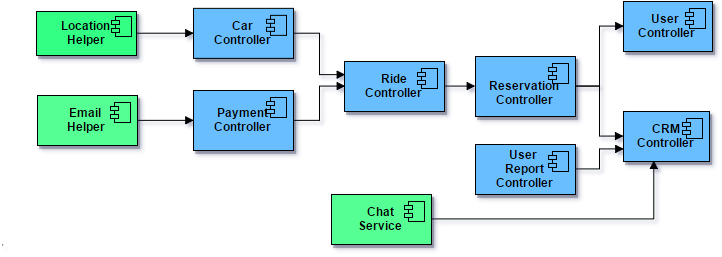
\includegraphics[width=1.4\textwidth]{ServerIntegrationSequence.png}}%
\caption {Server Components Integration}
\vspace*{0.5cm}
\end{figure} 

\paragraph{Client Tier:}
The Client Tier is based in two main components, User and CRM. Even if they are different they share many common functionalities including Login, Car Localization, Car Detail and Chat Service. They can be deployed simultaneously as they do not depend on each other and to test the logic subsystem from the Client side we can deploy one functionality at a time when all the dependencies have been met.

\newpage
\begin{figure}[h]
\centering
\vspace*{\fill}
\noindent\makebox[\textwidth]{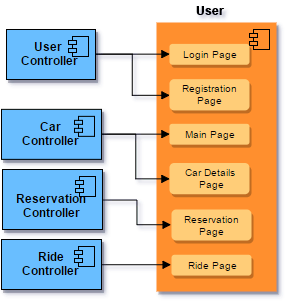
\includegraphics[width=0.45\textwidth]{UserComponentDependencies.png}}%
\caption {User Component Dependencies}
\vspace*{0.5cm}
\end{figure} 

\begin{figure}[h]
\centering
\vspace*{\fill}
\noindent\makebox[\textwidth]{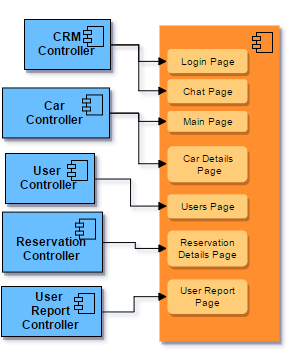
\includegraphics[width=0.45\textwidth]{CRMComponentDependencies.png}}%
\caption {CRM Component Dependencies}
\vspace*{0.5cm}
\end{figure}
 
\newpage
\subsubsection{Subsystem Integration Sequence}
As mentioned before our subsystems corresponging to the Data, Logic and Presentation Tier will be integrated in that order. Before integrating a subsystem all the components inside it must be integrated as well.
\begin{figure}[h]
\centering
\vspace*{\fill}
\noindent\makebox[\textwidth]{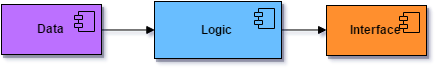
\includegraphics[width=0.9\textwidth]{SubsystemsDependencies.png}}%
\caption {Subsystem Integration Sequence}
\vspace*{0.5cm}
\end{figure}


\newpage
\section{Individual Steps and Test Description}
This section will include a detailed description on the sequence and tests to be performed on each component to be integrated. For each component we'll present individual function testing to secure the correctness and robustness of the function with respect to unexpected or invalid input. For integration testing we'll test if each of the component involved works as expected or if not, where does the error occur to determine critical points in the integration. The EIS Tier is considered to be implemented for the individual function testing. To get an overall picture of the Component functions and interfaces look at the Section 2 of the \textbf{DD}.
\par \textit{Note:} Null Input tests are considered for all applicable functions and these are considered to respond with a NullArgumentException unless expressed otherwise.
\subsection{Location Helper}
This component uses Google Maps API which locations use 2 float parameters, as many functions use the class Location we remind that, as explained in the DD, the Class consist in two floats, lat (latitude) and lon (longitude). All functions that accept Location as parameter will also be implemented to accept 2 floats as parameters. 
\newline
\newline
\textbf{Function:} isSafeParkingArea(Location) : bool
\begin{center}
\begin{tabular}{ | L{7cm} | L{5cm} | }
\hline
	\textit{Input}& \textit{Response}\\ \hline
	Invalid or Null Location & false \\ \hline
	Location valid inside the Valid parking area. Check with DB. & true \\ \hline
\end{tabular}
\end{center}

\textbf{Function:} getCloseRechargingStations(Location) : List\(<Location>\)
\begin{center}
\begin{tabular}{ | L{7cm} | L{5cm} | }
\hline
	\textit{Input}& \textit{Response}\\ \hline
	Invalid or Null Location & Empty List \\ \hline
	Location valid inside the Valid parking area. & Returns the list of available Recharging Stations closeby \\ \hline
\end{tabular}
\end{center}
\newpage 

\textbf{Function:} getBestRechargingStation(Location) : Location  \par
\textit{//Uses getCloseRechargingStations}
\begin{center}
\begin{tabular}{ | L{7cm} | L{5cm} | }
\hline
	\textit{Input}& \textit{Response}\\ \hline
	Invalid or Null Location & Null Location \\ \hline
	Location valid inside the Valid parking area. & Returns the best available Recharging station found by the Standard Deviation Algorithm  \\ \hline
\end{tabular}
\end{center}

\textbf{Function:} calculatePath(Location, Location) : List\(<Location>\)
\begin{center}
\begin{tabular}{ | L{6cm} | L{6cm} | }
\hline
	\textit{Input}& \textit{Response}\\ \hline
	Invalid or Null Location & Empty List \\ \hline
	Locations valid inside the Valid parking area. & Returns faster path found by the Google Maps API, if path not found returns Empty List \\ \hline
\end{tabular}
\end{center}

\subsection{Email Helper}
\textbf{Function:} sendRegistrationEmail(Email, Password) : void
\begin{center}
\begin{tabular}{ | L{6cm} | L{6cm} | }
\hline
	\textit{Input}& \textit{Response}\\ \hline
	Invalid Email & Password Delivery failed Exception \\ \hline
	Valid Email and Password & Registration Mail sent \\ \hline
\end{tabular}
\end{center}
\textbf{Function:} sendPaymentEmail(Email, Payment) : void
\begin{center}
\begin{tabular}{ | L{6cm} | L{6cm} | }
\hline
	\textit{Input}& \textit{Response}\\ \hline
	Invalid Email & Payment Delivery failed Exception \\ \hline
	Valid Email and Payment & Payment Mail sent \\ \hline
\end{tabular}
\end{center}

\subsection{Chat Service}
\textbf{Function:} requestCRMContact() : Id
\begin{center}
\begin{tabular}{ | L{6cm} | L{6cm} | }
\hline
	\textit{Input}& \textit{Response}\\ \hline
	None & Returns a vaild CRM Id that is available for contact, else returns Null \\ \hline
\end{tabular}
\end{center}
\newpage

\subsection{Car Controller}
Our system will not handle adding or deleting Cars in the DB so these operations will not be integrated. Just operations that search or change the state of the Car.
\textbf{Function:} reserveCar(CarId) : bool
\begin{center}
\begin{tabular}{ | L{6cm} | L{6cm} | }
\hline
	\textit{Input}& \textit{Response}\\ \hline
	Invalid or CarID not present & false - DB unchanged\\ \hline
	CarID already reserved & false - DB unchanged\\ \hline
	Valid CarID & true - Car marked as reserved in the DB\\ \hline
\end{tabular}
\end{center}

\textbf{Function:} enableCar(CarId) : bool
\begin{center}
\begin{tabular}{ | L{6cm} | L{6cm} | }
\hline
	\textit{Input}& \textit{Response}\\ \hline
	Invalid or CarID not present & false - DB unchanged\\ \hline
	Valid CarID & true - Car changed to enabled in the DB\\ \hline
\end{tabular}
\end{center}

\textbf{Function:} disableCar(CarId) : bool
\begin{center}
\begin{tabular}{ | L{6cm} | L{6cm} | }
\hline
	\textit{Input}& \textit{Response}\\ \hline
	Invalid or CarID not present & false - DB unchanged\\ \hline
	Valid CarID & true - Car changed to disabled in the DB\\ \hline
\end{tabular}
\end{center}
\textbf{Function:} getCloseCars(Location) : List\(<CarId>\) \par
\textit{Components:} LocationHelper
\begin{center}
\begin{tabular}{ | L{6cm} | L{6cm} | }
\hline
	\textit{Input}& \textit{Response}\\ \hline
	Invalid or Null Location & Empty List \\ \hline
	Locations valid & Returns List of Cars close in walking range to a given Location \\ \hline
\end{tabular}
\end{center}
\newpage

\subsection{Payment Controller}
\textbf{Function:} createPayment(Ammount, ExtraFees) : Payment \par
\begin{center}
\begin{tabular}{ | L{6cm} | L{6cm} | }
\hline
	\textit{Input}& \textit{Response}\\ \hline
	Invalid or Null Ammount & Null \\ \hline
	Valid Ammount & Creates Payment in the DB and returns the created Entity \\ \hline
\end{tabular}
\end{center}
\textbf{Function:} executeTransaction(Payment) : bool \par
\begin{center}
\begin{tabular}{ | L{6cm} | L{6cm} | }
\hline
	\textit{Input}& \textit{Response}\\ \hline
	Invalid or Null Payment & false, Payment not executed \\ \hline
	Valid Payment & true if Payment successfull \\ \hline
\end{tabular}
\end{center}

\subsection{Ride Controller}
\textbf{Function:} createRide(User, Car) : Ride \par
\textit{Components:} CarController
\begin{center}
\begin{tabular}{ | L{6cm} | L{6cm} | }
\hline
	\textit{Input}& \textit{Response}\\ \hline
	Invalid or Null Parameters & Null, Ride not created \\ \hline
	Valid Parameters & Creates Ride and marks Car as Ready in the DB, returns the created Entity\\ \hline
\end{tabular}
\end{center}
\textbf{Function:} startRide(RideId) : bool \par
\textit{Components:} CarController
\begin{center}
\begin{tabular}{ | L{6cm} | L{6cm} | }
\hline
	\textit{Input}& \textit{Response}\\ \hline
	Invalid or Null Ride & false, Ride not started \\ \hline
	Already started RideID & false \\ \hline
	Valid not started Ride & true, marks the Ride as started and the Car in Use\\ \hline
\end{tabular}
\end{center}
\textbf{Function:} stopRide(RideId) : bool \par
\textit{Components:} CarController
\begin{center}
\begin{tabular}{ | L{6cm} | L{6cm} | }
\hline
	\textit{Input}& \textit{Response}\\ \hline
	Invalid or Null Ride & false, Ride not stopped \\ \hline
	Already stopped RideID & false \\ \hline
	Valid started Ride & true, marks the Ride as stopped and the Car Ready\\ \hline
\end{tabular}
\end{center}
\textbf{Function:} CalculateFee(RideId) : Payment \par
\textit{Components:} PaymentController
\begin{center}
\begin{tabular}{ | L{6cm} | L{6cm} | }
\hline
	\textit{Input}& \textit{Response}\\ \hline
	Invalid or Null Ride & Null, Fee not calculated\\ \hline
	Not stopped RideID & Null, Fee has to be calculated on a stopped Ride \\ \hline
	Valid stopped Ride & Calculates all the Extra Fees appliable in the Ride and creates Payment with the Payment Controller.\\ \hline
\end{tabular}
\end{center}

\subsection{Reservation Controller}
\textbf{Function:} createReservation(UserID, CarID) : Reservation \par
\textit{Components:} CarController
\begin{center}
\begin{tabular}{ | L{6cm} | L{6cm} | }
\hline
	\textit{Input}& \textit{Response}\\ \hline
	Invalid or Null Parameters & Null, Reservation not created \\ \hline
	Valid Parameters & Creates Reservation and marks Car as Reserved in the DB, returns the created Entity\\ \hline
\end{tabular}
\end{center}
\textbf{Function:} cancelReservation(ReservationID) : bool \par
\textit{Components:} CarController
\begin{center}
\begin{tabular}{ | L{6cm} | L{6cm} | }
\hline
	\textit{Input}& \textit{Response}\\ \hline
	Invalid or Null ReservationID & false, Reservation not canceled \\ \hline
	Already canceled or confirmed Reservation RideID & false, Reservation has to be pending to be canceled \\ \hline
	Valid Reservation & true, marks the Reservation as canceled and the Car as Available\\ \hline
\end{tabular}
\end{center}
\textbf{Function:} confirmReservation(ReservationID) : bool \par
\textit{Components:} RideController
\begin{center}
\begin{tabular}{ | L{6cm} | L{6cm} | }
\hline
	\textit{Input}& \textit{Response}\\ \hline
	Invalid or Null ReservationID & false, Ride not stopped \\ \hline
	Already canceled or confirmed ReservationID & false, Reservation has to be pending to be confirmed\\ \hline
	Valid started Reservation & true, Creates the corresponding Ride for the Reservation, marks the Reservation as confirmed\\ \hline
\end{tabular}
\end{center}

\subsection{User Report Controller}
\textbf{Function:} createUserReport(CRMID, UserID, CarID) : UserReport \par
\begin{center}
\begin{tabular}{ | L{6cm} | L{6cm} | }
\hline
	\textit{Input}& \textit{Response}\\ \hline
	Invalid or Null Parameters & Null, UserReport not created \\ \hline
	Valid Parameters & Creates UserReport, returns the created Entity\\ \hline
\end{tabular}
\end{center}

\subsection{User Controller}
Functions of the User (and CRM) Controller integrate with functions of other Controllers since they change the status of the User and then relegate the changes of the other Entities to the respective Controllers. For the functions that were presented on the previous Controllers we will reduce repetitiveness by reducing the details of already explained output for functions. Look at the DD for detailed information of the interaction between components. \par
\textbf{Function:} registerUser(User Parameters) : User \par
\textit{Components:} EmailHelper
\textit{//Look up the RASD for the User Parameters}
\begin{center}
\begin{tabular}{ | L{6cm} | L{6cm} | }
\hline
	\textit{Input}& \textit{Response}\\ \hline
	Invalid or Null Parameters & Null, User not created \\ \hline
	Valid Parameters & Creates User in the DB, sends Password mail and returns the created Entity\\ \hline
\end{tabular}
\end{center}
\textbf{Function:} logIn(UserID, Password) : bool \par
\begin{center}
\begin{tabular}{ | L{6cm} | L{6cm} | }
\hline
	\textit{Input}& \textit{Response}\\ \hline
	Invalid or Null Parameters & false, Invalid User Exception\\ \hline
	Already logged in User & false, User already logged in Exception\\ \hline
	Valid Parameters on DB & true, Logs in User into the System \\ \hline
\end{tabular}
\end{center}
\textbf{Function:} logOut(UserID) : bool \par
\begin{center}
\begin{tabular}{ | L{6cm} | L{6cm} | }
\hline
	\textit{Input}& \textit{Response}\\ \hline
	Invalid or Null Parameters & false, Invalid User Exception\\ \hline
	Already logged out User & false, User already logged out Exception\\ \hline
	Valid Parameters on DB & true, Logs out User from the System \\ \hline
\end{tabular}
\end{center}
\textbf{Function:} reserveCar(UserID, CarID) : ReservationID \par
\textit{Components:} ReservationController
\begin{center}
\begin{tabular}{ | L{6cm} | L{6cm} | }
\hline
	\textit{Input}& \textit{Response}\\ \hline
	Invalid or Null Parameters & Null, Reservation not created and status not changed\\ \hline
	Already Reserved Car or User & false, Car and User cannot have more than one Reservation at a time\\ \hline
	Valid Parameters & true, Creates Reservation binds ReservationID to the User \\ \hline
\end{tabular}
\end{center}
\textbf{Function:} confirmReservation(UserID, ReservationID) : RideID \par
\textit{Components:} ReservationController
\begin{center}
\begin{tabular}{ | L{6cm} | L{6cm} | }
\hline
	\textit{Input}& \textit{Response}\\ \hline
	Invalid or Null Parameters & Null, Ride not created\\ \hline
	Already confirmed Reservation & false, Ride not created\\ \hline
	User with already active Ride & false, Ride not created\\ \hline
	Valid User and Reservation& true, Creates Ride and binds RideID to the User \\ \hline
\end{tabular}
\end{center}
\textbf{Function:} cancelReservation(UserID, ReservationID) : bool \par
\textit{Components:} ReservationController
\begin{center}
\begin{tabular}{ | L{6cm} | L{6cm} | }
\hline
	\textit{Input}& \textit{Response}\\ \hline
	Invalid or Null Parameters & false, Invalid Parameters Exception\\ \hline
	User not binded to Reservation & false, Invalid Reservation Exception\\ \hline
	Valid User and Reservation& true, unbinds Reservation form User\\ \hline
\end{tabular}
\end{center}
\textbf{Function:} endRide(UserID, RideID) : bool \par
\textit{Components:} RideController
\begin{center}
\begin{tabular}{ | L{6cm} | L{6cm} | }
\hline
	\textit{Input}& \textit{Response}\\ \hline
	Invalid or Null Parameters & false, Invalid Parameters Exception\\ \hline
	User not binded to Ride & false, Invalid Ride Exception\\ \hline
	Valid User and Ride& true, stops the ride and calculates and executes the Payment\\ \hline
\end{tabular}
\end{center}
\newpage

\subsection{CRM Controller}
\textbf{Function:} logIn(CRMID, Password) : bool \par
\begin{center}
\begin{tabular}{ | L{6cm} | L{6cm} | }
\hline
	\textit{Input}& \textit{Response}\\ \hline
	Invalid or Null Parameters & false, Invalid CRM Exception\\ \hline
	Already logged in CRM & false, CRM already logged in Exception\\ \hline
	Valid Parameters on DB & true, Logs in CRM into the System \\ \hline
\end{tabular}
\end{center}
\textbf{Function:} logOut(CRMID) : bool \par
\begin{center}
\begin{tabular}{ | L{6cm} | L{6cm} | }
\hline
	\textit{Input}& \textit{Response}\\ \hline
	Invalid or Null Parameters & false, Invalid CRMID Exception\\ \hline
	Already logged out CRMID & false, CRMID already logged out Exception\\ \hline
	Valid Parameters on DB & true, Logs out CRMID from the System \\ \hline
\end{tabular}
\end{center}
\textbf{Function:} createUserReport(CRMID, UserID, CarID, CarStatus) : UserReport \par
\textit{Components:} UserReportController, CarController
\begin{center}
\begin{tabular}{ | L{6cm} | L{6cm} | }
\hline
	\textit{Input}& \textit{Response}\\ \hline
	Invalid or Null Parameters & Null, UserReport not created\\ \hline
	Valid Parameters & true, Creates UserReport and changes the CarStatus if necessary\\ \hline
\end{tabular}
\end{center}
\textbf{Function:} cancelReservation(UserID, ReservationID) : bool \par
\textit{Components:} ReservationController
\begin{center}
\begin{tabular}{ | L{6cm} | L{6cm} | }
\hline
	\textit{Input}& \textit{Response}\\ \hline
	Invalid or Null Parameters & false, Invalid Parameters Exception\\ \hline
	Valid User and Reservation& true, cancels Reservation\\ \hline
\end{tabular}
\end{center}
\textbf{Function:} createReservation(UserID, CarID) : bool \par
\textit{Components:} ReservationController
\begin{center}
\begin{tabular}{ | L{6cm} | L{6cm} | }
\hline
	\textit{Input}& \textit{Response}\\ \hline
	Invalid or Null Parameters & false, Invalid Parameters Exception\\ \hline
	Valid User and Reservation& true, creates new Reservation for User\\ \hline
\end{tabular}
\end{center}
\textbf{Function:} endRide(UserID, RideID) : bool \par
\textit{Components:} RideController
\begin{center}
\begin{tabular}{ | L{6cm} | L{6cm} | }
\hline
	\textit{Input}& \textit{Response}\\ \hline
	Invalid or Null Parameters & false, Invalid Parameters Exception\\ \hline
	Valid User and Reservation& true, cancels Ride\\ \hline
\end{tabular}
\end{center}
\subsection{User Component}
\textbf{Function:} logInUser(UserName, Password) : bool \par
\textit{Components:} UserController
\begin{center}
\begin{tabular}{ | L{6cm} | L{6cm} | }
\hline
	\textit{Input}& \textit{Response}\\ \hline
	Invalid or Null Parameters & false\\ \hline
	Valid Parameters & true if UserController logs in the User\\ \hline
\end{tabular}
\end{center}
\textbf{Function:} logOutUser(UserName) : bool \par
\textit{Components:} UserController
\begin{center}
\begin{tabular}{ | L{6cm} | L{6cm} | }
\hline
	\textit{Input}& \textit{Response}\\ \hline
	Invalid or Null Parameters & false\\ \hline
	Valid Parameters & true if UserController logs out the User\\ \hline
\end{tabular}
\end{center}
\textbf{Function:} registerUser(UserParameters) : bool \par
\textit{Components:} UserController
\begin{center}
\begin{tabular}{ | L{6cm} | L{6cm} | }
\hline
	\textit{Input}& \textit{Response}\\ \hline
	Invalid or Null Parameters & false\\ \hline
	Valid Parameters & true if UserController registers the User\\ \hline
\end{tabular}
\end{center}

\textbf{Function:} searchNearbyCars(Location) : List\(<Car>\) \par
\textit{Components:} CarController
\begin{center}
\begin{tabular}{ | L{6cm} | L{6cm} | }
\hline
	\textit{Input}& \textit{Response}\\ \hline
	Invalid or Null Location & Shows all Cars in the MainPage Map\\ \hline
	Valid Parameters & Shows the nearby Cars in the MainPage Map\\ \hline
\end{tabular}
\end{center}
\newpage

\textbf{Function:} reserveCar(UserID, CarID) : bool \par
\textit{Components:} UserController
\begin{center}
\begin{tabular}{ | L{6cm} | L{6cm} | }
\hline
	\textit{Input}& \textit{Response}\\ \hline
	Invalid or Null Parameters & false\\ \hline
	Valid Parameters & true if UserController was able to reserve the Car\\ \hline
\end{tabular}
\end{center}
\textbf{Function:} cancelReservation(UserID, ReservationID) : bool \par
\textit{Components:} UserController
\begin{center}
\begin{tabular}{ | L{6cm} | L{6cm} | }
\hline
	\textit{Input}& \textit{Response}\\ \hline
	Invalid or Null Parameters & false\\ \hline
	Valid Parameters & true if UserController was able to cancel Reservation\\ \hline
\end{tabular}
\end{center}
\textbf{Function:} confirmlReservation(UserID, ReservationID) : bool \par
\textit{Components:} UserController
\begin{center}
\begin{tabular}{ | L{6cm} | L{6cm} | }
\hline
	\textit{Input}& \textit{Response}\\ \hline
	Invalid or Null Parameters & false\\ \hline
	Valid Parameters & true if UserController was able to confirm Reservation\\ \hline
\end{tabular}
\end{center}
\textbf{Function:} endRide(UserID, RideID) : bool \par
\textit{Components:} UserController
\begin{center}
\begin{tabular}{ | L{6cm} | L{6cm} | }
\hline
	\textit{Input}& \textit{Response}\\ \hline
	Invalid or Null Parameters & false\\ \hline
	Valid Parameters & true if UserController was able to end the Ride\\ \hline
\end{tabular}
\end{center}
\textbf{Function:} findLocation(Location) : List\(<Location>\) \par
\textit{Components:} LocationHelper
\begin{center}
\begin{tabular}{ | L{6cm} | L{6cm} | }
\hline
	\textit{Input}& \textit{Response}\\ \hline
	Invalid Location & Empty Path\\ \hline
	Valid Parameters & shows the desired path in the Ride Map\\ \hline
\end{tabular}
\end{center}
\newpage

\textbf{Function:} activateMoneySavingOption(Location) : Location \par
\textit{Components:} LocationHelper
\begin{center}
\begin{tabular}{ | L{6cm} | L{6cm} | }
\hline
	\textit{Input}& \textit{Response}\\ \hline
	Invalid Location & Null Location\\ \hline
	Valid Parameters & shows the best Re-Charging Station in the Ride Map\\ \hline
\end{tabular}
\end{center}

\subsection{CRM Component}
\textbf{Function:} logInCRM(CRMID, Password) : bool \par
\textit{Components:} CRMController
\begin{center}
\begin{tabular}{ | L{6cm} | L{6cm} | }
\hline
	\textit{Input}& \textit{Response}\\ \hline
	Invalid or Null Parameters & false\\ \hline
	Valid Parameters & true if CRMController logs in the CRM\\ \hline
\end{tabular}
\end{center}
\textbf{Function:} logOutCRM(CRMName) : bool \par
\textit{Components:} CRMController
\begin{center}
\begin{tabular}{ | L{6cm} | L{6cm} | }
\hline
	\textit{Input}& \textit{Response}\\ \hline
	Invalid or Null Parameters & false\\ \hline
	Valid Parameters & true if CRMController logs out the User\\ \hline
\end{tabular}
\end{center}
\textbf{Function:} findCars(Location, CarStatus) : List\(<Car>\) \par
\textit{Components:} CarController
\begin{center}
\begin{tabular}{ | L{6cm} | L{6cm} | }
\hline
	\textit{Input}& \textit{Response}\\ \hline
	Invalid Parameters & Empty List\\ \hline
	Valid Parameters & shows the List of desired Cars\\ \hline
\end{tabular}
\end{center}
\textbf{Function:} findUsers(UserStatus) : List\(<User>\) \par
\textit{Components:} UserController
\begin{center}
\begin{tabular}{ | L{6cm} | L{6cm} | }
\hline
	\textit{Input}& \textit{Response}\\ \hline
	Invalid Parameters & Empty List\\ \hline
	Valid Parameters & shows the List of desired Users\\ \hline
\end{tabular}
\end{center}
\newpage

\textbf{Function:} findReservations(UserID, CarID, ReservationStatus) : \par List\(<Reservation>\) \par
\textit{Components:} ReservationController
\begin{center}
\begin{tabular}{ | L{6cm} | L{6cm} | }
\hline
	\textit{Input}& \textit{Response}\\ \hline
	Invalid Parameters & Empty List\\ \hline
	Valid Parameters & shows the List of desired Reservations\\ \hline
\end{tabular}
\end{center}
\textbf{Function:} findRides(UserID, CarID, RideStatus) : List\(<Ride>\) \par
\textit{Components:} RideController
\begin{center}
\begin{tabular}{ | L{6cm} | L{6cm} | }
\hline
	\textit{Input}& \textit{Response}\\ \hline
	Invalid Parameters & Empty List\\ \hline
	Valid Parameters & shows the List of desired Rides\\ \hline
\end{tabular}
\end{center}
\textbf{Function:} findPayments(UserID, CarID) : List\(<Payments>\) \par
\textit{Components:} PaymentController
\begin{center}
\begin{tabular}{ | L{6cm} | L{6cm} | }
\hline
	\textit{Input}& \textit{Response}\\ \hline
	Invalid Parameters & Empty List\\ \hline
	Valid Parameters & shows the List of desired Payments\\ \hline
\end{tabular}
\end{center}

\textbf{Function:} findUserReports(UserID, CarID, CRMID) : List\(<UserReports>\) \par
\textit{Components:} UserReportController
\begin{center}
\begin{tabular}{ | L{6cm} | L{6cm} | }
\hline
	\textit{Input}& \textit{Response}\\ \hline
	Invalid Parameters & Empty List\\ \hline
	Valid Parameters & shows the List of desired UserReports\\ \hline
\end{tabular}
\end{center}


\subsection{Car Component}
\textbf{Function:} getLocation() : Location \par
\begin{center}
\begin{tabular}{ | L{6cm} | L{6cm} | }
\hline
	\textit{Input}& \textit{Response}\\ \hline
	None & returns Car Location\\ \hline
\end{tabular}
\end{center}
\textbf{Function:} getNumberOfPassengers() : int \par
\begin{center}
\begin{tabular}{ | L{6cm} | L{6cm} | }
\hline
	\textit{Input}& \textit{Response}\\ \hline
	None & returns the current Number of Passengers in the Car\\ \hline
\end{tabular}
\end{center}
\textbf{Function:} getBatteryStatus() : float \par
\begin{center}
\begin{tabular}{ | L{6cm} | L{6cm} | }
\hline
	\textit{Input}& \textit{Response}\\ \hline
	None & returns the current Battery Status in percentage (0-100)\\ \hline
\end{tabular}
\end{center}
\textbf{Function:} isPluggedIn() : bool \par
\begin{center}
\begin{tabular}{ | L{6cm} | L{6cm} | }
\hline
	\textit{Input}& \textit{Response}\\ \hline
	None & returns true if the Car is plugged in a Re-Charging Station, false otherwise\\ \hline
\end{tabular}
\end{center}
\textbf{Function:} lockCar() : bool \par
\begin{center}
\begin{tabular}{ | L{6cm} | L{6cm} | }
\hline
	\textit{Input}& \textit{Response}\\ \hline
	None & returns true if Car was Locked\\ \hline
\end{tabular}
\end{center}
\textbf{Function:} unlockCar() : bool \par
\begin{center}
\begin{tabular}{ | L{6cm} | L{6cm} | }
\hline
	\textit{Input}& \textit{Response}\\ \hline
	None & returns true if Car was Unlocked\\ \hline
\end{tabular}
\end{center}
\newpage
\section{Performance Analysis}

Even tough the performance analysis is evaluated within the system as a whole, it was agreed that while testing the components, the isolated performance will be taken into account, as to correct unacceptable behavior, such as too slow response time, as soon as possible. 

The aim of the performance analysis is to check the reliability of the application under normal usage conditions, providing benchmarks and identifying the response time, utilization and throughput of the application. So, for this test, the expected workload should be considered as in terms of the biggest city where the application will be implemented, taking into account an average usage for a long period with peaks of heavy traffic. 

Both the server side and the client side can affect the performance of the application. For the client side,  it is necessary to consider the performance of all the different interfaces. Particularly, the mobile application, the web application and the screen inside the car should all have satisfactory behavior, considering all kinds of users that can operate each of them. 

Some important requirements to be evaluated:
\begin{itemize}
\item[-] For the mobile application it is considered that the target public of the app can have any kind of Smartphone. So, the test will be made in low-range devices. This includes low ram availability, small internal space allocation and low processing power capacity.
\item[-] All the interfaces need to respond properly with slow network situations, and be reliable in situations of unstable network. 

\end{itemize}
\newpage


\section{Required Tools and Test Equipment}
\subsection{Tools}

In order to guarantee the most reliable system possible, when integrating components all the individual tests will be carried out once again, to make sure the integration did not cause new bugs to occur. For this reason, all the used programs provide tests automation tools, minimizing the rework. 

The tools chosen for the Java EE and the EIS tiers were specifically three and each has it’s own scope of tests.

\begin{itemize}
\item First, the \textbf{JUnit Framework} will take care of the individual components testing. This is basically a way to certify that results produced by the components matches the theoretical value.

\item Secondly, the \textbf{Arquillian Framework} helps keeping the integration testing simple. Testing the components of an application is challenging, so this framework focus on the interaction with the system, providing tools to check that the right components are being injected and the interactions with the database are occurring in a normal way. 

\item Finally,\textbf{Jmeter Framework} brings the application closer to the real world by performing load tests and performance tests. This tool provides emulations of loads on the server, network and objects providing solid data to analyze the overall performance of the systems under various conditions.
\end{itemize}
However, it is still necessary to  test components withheld in the Client tier,  specifically the mobile applications. In this matter, it will be used tools provided with each platform (IOS and Android have their own performance analysis tool that comes along with the SDK of the plataform). Also as stated in the previous session, particularly harsh situations as low battery, bad network coverage and low available memory need to be taken into account. 

These tools ensure that every aspect of the application is tested in the proper way and provide all the necessary features to accomplish the proposed points of this document.
\newpage

\subsection{Test Equipment}

In some previous sections, characteristics of the devices in which the application needs to operate successfully have been discussed. They were always pessimistic, assuming that low-range smarphones, with limited functionalities were being used. However, this is only part of the testing devices, most users own better smarphones than the ones described. And even tough the older devices should be supported, the application must be better optimized for the majority of the public.

Therefore, for the Android application, for each available screen size in the market (including smarphones and tablets), it will be necessary to execute the tests for a low-range and a mid-range device.  

When using a low-range device, the characteristics to keep in mind are a single core with slow processor clock (preferably less then 1 ghz), and less then 1gb of ram. As for mid-range, it can be a dual core with up to 2ghz of clock, and 2gb of ram.  

In the IOS the specifications of the devices only vary within the different models, so at least one smarpthone and tablet of the IOS family need to be available for testing.

For the devices above described it will be carried out tests with the native mobile application and the mobile version of the web application. This is to ensure a broader number of devices and ways of accessing the application is covered.

Changing the scope from the mobile applications to the web browser client, a small number of notebooks and computers are also to be used, here the specifications of the devices are not important, but different browsers need to be installed in each of them. 

The last category of devices that will be used are in respect to the screen inside the car.  The tests will be carried out in android based devices, with different processing power and RAM availability. The results will be used to choose which model is to be deployed to all cars as to minimize the costs while keeping the necessary quality.

Finally, a identical server structure of the one used for the final deployment needs to be available. Although this is not yet completely defined, the test should recreate a realistic environment, using the same cloud infrastructure, Operating System, Java Enterprise Application server, and DBMS. 
\newpage



\section{Required Program Stubs and Test Data}

\subsection{Program Stubs and Drivers}
It was chosen as integration testing strategy the Bottom-up type. Due that it will be necessary the employment of Drivers to act as callers of the methods/components that need to be tested. The drivers that are listed below will compose the integration testing.
\begin{itemize}
\item \textbf{DBMS Driver:} Being the first in need to be integrated, the DBMS Driver will call the methods of the DBMS to test the interaction of the DBMS with the subsystems.

\item \textbf{Location Helper Driver:} Although this driver has the main function to test the interaction among Location Helper and the Car Controller it will test also functions such as of the Standard Deviation Algorithm used in the function ‘getBestRechargingStation’ and the interaction of the functions with the Google Maps API.

\item \textbf{Email Helper Driver:} This driver will test the interaction of the Email Helper with Payment Controller and will test the functionality by calling the components of the Helper as sending the password by e-mail for the user.

\item \textbf{Chat Service Driver:}This driver will test the interaction of the component of the Chat Service with the CRM Controller by calling the method of the Chat Service.

\item \textbf{Car Controller Driver:} This driver will test the interaction of the  Car Controller with the Location Helper and with the Ride Controller by calling the methods of the Car Controller. In this case one method of the car controller will call as stipulated the Location Helper.  

\item \textbf{Payment Controller Driver:} This driver will test the interaction of the Payment Controller with the Email Helper and with the Ride Controller by calling the methods of the Payment Controller. In this case one method of the car controller will call as stipulated the Email Helper.  
\item \textbf{Ride Controller Driver:} This driver will directly test the interaction of the Ride Controller with the Car Controller, Payment Controller and with the Reservation Controler.Upon the calling of the methods of the Ride Controller the connection of it with the Reservation Controlleras well as their relation with the past components(Car Controller, Payment Controller) will be tested.
\item \textbf{Reservation Controller Driver:} This driver will test the interaction of the Reservation Controller with the Ride Controller, User Controller and with the CRM Controller by calling the methods of the Reservation Controller. 


\item \textbf{User Report Controller Driver:}  This driver will test the interaction of the User Report Controller with the CRM Controller by calling the methods of the User Report Controller. 

\item \textbf{User Controller Driver:} This driver will test the interaction of the User Controller with the Reservation Controller by calling the methods of the User Controller. 


\item \textbf{CRM Controller Driver: } This driver will test the interaction of the CRM Controller with the User Report Controller and the Chat Service by calling the methods of the User Controller. 
\end{itemize}  

\subsection{Test Data}
It will be necessary some set of data for the testing phase and they will be:
\begin{itemize}
\item A list with valid and invalid  locations. Also the list must test the following aspects of the system:
\begin{itemize}
     \item Null objects
     \item Null fields
     \item Location not in the required format
   \end{itemize}
\item A list with valid and invalid Users for the User Component. Also the list must test the following aspects of the system:
\begin{itemize}
     \item Null objects
     \item Null fields
     \item User already registered
     \item Invalid E-mail address
     \item Format of the driving license is not suitable   \end{itemize}
\item A list with valid and invalid CRM operators for the CRM component. Furthermore the list must contain:
\begin{itemize}
     \item Null objects
     \item Null fields
     \item Available status of the CRM operator
     \item Unavailable status of the CRM operator   
     \end{itemize}

\end{itemize}  
\newpage
\section{Effort Spent}
\begin{tabular}{ | c | c | c | c | }
\hline
	\textbf {Date} & \textbf {Domenico} & \textbf {Caio} & \textbf {Matheus} \\ \hline
	27/12/16& 2h & 2h & 2h  \\ \hline
	28/12/16& - & - & - \\ \hline
	29/12/16& 1h & - & - \\ \hline
	30/12/16& 2h & - & - \\ \hline
	31/12/16& - & - & - \\ \hline
	01/01/17& - & - & - \\ \hline
	02/01/17& 2h & - & - \\ \hline
	03/01/17& 2h & - & - \\ \hline
	04/01/17& 2h & - & - \\ \hline
	05/01/17& - & - & - \\ \hline
	06/01/17& - & - & - \\ \hline
	07/01/17& - & - & - \\ \hline
	08/01/17& - & - & 5h \\ \hline
	09/01/17& - & - & 4h \\ \hline
	10/01/17& 2h & 2h & - \\ \hline
	11/01/17& 2h & 5h & - \\ \hline
	12/01/17& - & 5h & - \\ \hline
	13/01/17& - & - & - \\ \hline
	14/01/17& - & - & - \\ \hline
\end{tabular}
\newpage

\section{Changelog}
As the project and design decisions may change during the development this document is also prone to change.
We'll document every version in this part.
\begin{itemize}
\item \textbf {Version 1.1:} 15/01/2017
\end{itemize}
\end{document}
